\chapter{Optical Activity in Plasmonic Metasurfaces}\label{sec:results:OAinPlanarNanohelices}

Sections of this chapter have been copied verbatim from the (published) manuscript \textit{``Second Harmonic Generation Optical Rotation Solely Attributable to Chirality in Plasmonic Metasurfaces''}, Joel~T.~Collins et. al. \cite{Collins2018b}.
V. K. Valev designed the nonlinear experimental setup. A.G.Mark fabricated the samples. SHG data were collected by myself, and D. C. Hooper. Linear optical data were collected by myself and C. Kuppe. I analysed both the SHG and linear data. Tensor analysis and analytical verification of experimental results were performed by myself. I produced the manuscript draft on which this chapter is based.

\bigskip \noindent
As discussed in section~\ref{sec:background:Chirality:anisotropy}, both linear and nonlinear optical rotation can occur even in achiral structures, if the structure is birefringent due to anisotropy, making pure chiral information difficult to obtain~\cite{Hooper2017}. 
Crucially however, chiroptical effects resulting from anisotropy in planar nanomaterials exhibit a strong dependence on structural orientation about the surface normal.
Here we report large second-harmonic generation optical rotation of $\pm\SI{45}{\degree}$, due to intrinsic chirality in a highly anisotropic helical metamaterial. 
The SHG \emph{intensity} is found to depend strongly on the structural anisotropy, however even at oblique incidence the SHG-OR is invariant as the sample is rotated about the surface normal. 
The results show that by tuning the geometry of anisotropic nanostructures, the interaction between anisotropy, chirality, and experiment geometry can allow greater control over the chiroptical properties of plasmonic metamaterials.

\section{Introduction}\label{sec:results:OAinPlanarNanohelices:introduction}
In this set of experiments, we made use of chiral optical metamaterials (section~\ref{sec:background:Plasmonics:Metamaterials}), whose properties are determined by both the choice of materials, and their geometry. Previously, large plasmon-enhanced linear CD and OR effects have been reported in chiral metamaterials \cite{Decker2007, Papakostas2003, Kuwata-Gonokami2005a, Plum2007, Gansel2011}.
Because CD and OR originate from the real and imaginary part of the refractive index, respectively, the two effects are linked by the Kramers-Kronig transforms (section~\ref{sec:background:Chirality:Chiroptics}).
However, this link is not necessary for nonlinear chiroptical effects; since nonlinear CID and OR do not result from the real and imaginary parts of a single complex number.

For second harmonic generation (SHG), the two nonlinear chiroptical effects SHG-CID and SHG-OR are fundamentally different from, and can be highly complementary to, linear chiroptical effects. For the latter, interacting parallel components of electric and magnetic dipoles are strictly necessary. This necessity is lifted in the nonlinear case. Since SHG is a three-wave mixing process, chiroptical effects can arise from the 3D chiral arrangement of electric dipoles only~\cite{verbiest2009second}. 
SHG chiroptical effects can also originate from the interaction between electric and magnetic dipoles, as well as between electric dipoles and quadrupoles. This specificity allows SHG to discriminate between two principal models of chirality~\cite{Fischer2005a}: Kuhn's ``chirally-coupled dipoles''~\cite{Kuhn1930} and Kauzmann's ``one electron on a helix''~\cite{Maki1996, Kauzmann1957a} models. More precisely, the two can be separated by measuring SHG-OR. 

Whereas SHG-CID has been demonstrated from numerous chiral nanomaterials \cite{Hooper2017, Mamonov2017, Chen2016, Kolkowski2015, Belardini2014}, far less attention has been devoted to SHG-OR. Previous studies have demonstrated SHG-OR in plasmonic nanostructures, where the origin of the effect can be ambiguous~\cite{Romain2017, Ren2012a, Mamonov2012}, since SHG-OR can originate from both intrinsic chirality and anisotropy. An unambiguously chiral origin of SHG-OR has not been previously reported in nano/meta-materials. 

\section{Results}\label{sec:results:OAinPlanarNanohelices:results}
Here, we demonstrate clear SHG-OR in plasmonic metamaterials, which is due to intrinsic chirality; the SHG-OR angle does not depend on the sample rotation angle and it reverses upon mirroring the geometry. Conversely, for the same sample, the linear OR angle depends strongly on the rotation of the sample, which demonstrates a dominant contribution from anisotropy rather than chirality, in the linear case. Moreover, we show that SHG-OR can also be dominantly sensitive to the anisotropy of the samples, depending on the experimental geometry and on the particular values of the nonlinear susceptibility tensor components involved. 

The samples used in these experiments are arrays of hexagonally-arranged Au:Cu (80:20) nanohelices, fabricated by A.G.Mark using a glancing-angle shadow growth method \cite{Gibbs2014}. The structures are shown schematically and in a cross-sectional SEM image in figure~\ref{fig:results:OAinPlanarNanohelices:setup}a and figure~\ref{fig:results:OAinPlanarNanohelices:setup}(b) respectively. 
Only one handedness of the structures is shown, however both left- and right-handed nanohelices were investigated. The individual nanohelices have a pitch of $\SI{37}{\nano\m}$, and height of $\SI{81}{\nano\m}$, a wire thickness of $\SI{18}{\nano\m}$, and the nanohelices have an inner and outer diameter of $\SI{28}{\nano\m}$ and $\SI{55}{\nano\m}$, respectively. Consequently, the structures are substantially sub-wavelength ($\approx\lambda/10$, at 800 nm).
The experimental setup (shown schematically in figure~\ref{fig:results:OAinPlanarNanohelices:setup}c) was designed to precisely measure the polarisation of SHG emission from the samples. 

$\SI{8.4}{\milli\watt}\pm\SI{0.1}{\milli\watt}$ of pulsed light centred at $\SI{800}{\nano\m}$ ($\SI{62}{\kilo\watt}$ peak power, appendix~\ref{sec:appendix:hardware:maitai}) was directed to a half-wave plate and rotated to a specific linear polarisation angle. An RG665 long pass filter removed any existing SHG from the beam, before an achromatic lens focused the $\SI{800}{\nano\m}$ light onto our sample at $\SI{45}{\deg}$ incidence. A BG39 filter then removed reflected $\SI{800}{\nano\m}$ light, passing only the $\SI{400}{\nano\m}$ SHG emission which was then collimated by another lens. The SHG emission then passed through an analysing polariser, before being focused onto a photomultiplier tube (PMT). The PMT output is pre-amplified and sent to an SRS SR400 Gated Photon Counter. 
By varying both the sample azimuthal rotation angle and the analysing polariser angle, a heatmap is produced. The latter shows the intensity of SHG emission, as a function of both sample rotation (along the $y$-axis) and analyser rotation (along the $x$-axis). 

\begin{figure}[htb!]	
    \centering	
    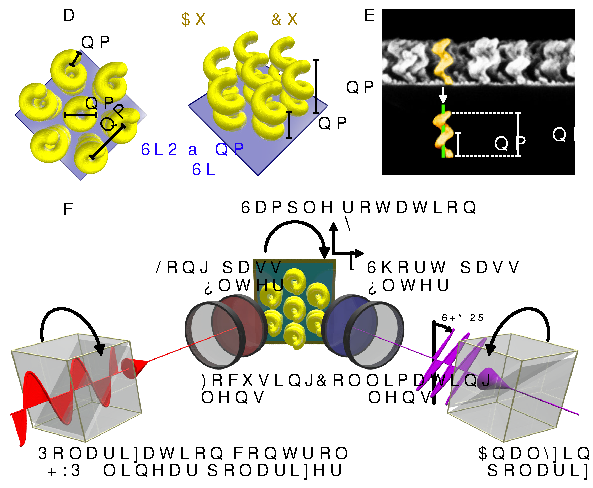
\includegraphics[scale=1.0]{./figures/results/OAinPlanarNanohelices/setup.pdf}
    \caption{\label{fig:results:OAinPlanarNanohelices:setup}
    \textbf{a)} Schematic diagram of one handedness of nanohelix array, showing structure spacing $\SI{55}{\nano\m}$, height $\SI{81}{\nano\m}$, and pitch $\SI{37}{\nano\m}$. \textbf{b)} Side-on SEM of the metamaterial surface, of the same handedness. A single helix has been highlighted for clarity. \textbf{c)} Schematic of experimental setup, showing S-polarised $\SI{800}{\nano\m}$ incident light. For optical rotation measurements, the analysing polariser is continuously rotated, for a series of sample azimuthal rotations.}	
\end{figure}

Figure~\ref{fig:results:OAinPlanarNanohelices:s_data} shows SHG hotspots corresponding to the polarisation of SHG emission as the sample is rotated. The green markers on Figure~\ref{fig:results:OAinPlanarNanohelices:s_data} show the angle of SHG polarisation for each sample rotation angle. Relative to the incoming S-polarised (perpendicular to the plane of incidence) light, an SHG-OR of approximately $+\SI{45}{\degree}$ is observed for the left-handed structures. Importantly, the SHG-OR angle does not change significantly over regions of strong SHG emission.
Moreover, upon measuring the right-handed structures, the SHG-OR reverses to approximately $-\SI{45}{\degree}$. While the data for the right-handed structure are noisier due to slight sample damage, the results are still clear. The reversal is exactly as expected for SHG-OR due to intrinsic chirality. The intensity of SHG emission does vary sinusoidally with rotation, suggesting a dipole coupling between the incident light and the end terminations of the nanohelices. After coupling into the structures via the end termination, the polarisation of light is then rotated by the intrinsic chirality of the helical structure.


\begin{figure}[htb!]	
    \centering	
    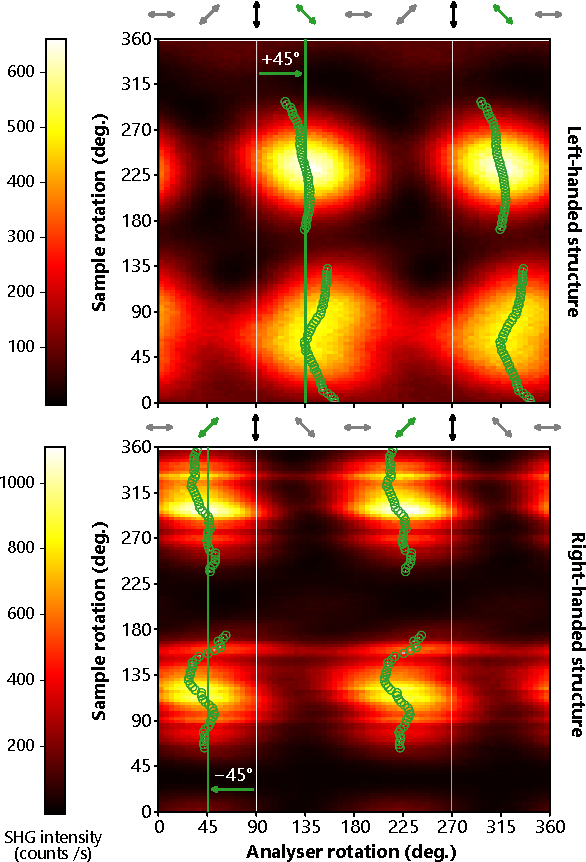
\includegraphics[scale=1]{./figures/results/OAinPlanarNanohelices/s_data.pdf}

    \caption{\label{fig:results:OAinPlanarNanohelices:s_data}
    SHG optical rotation heatmaps for both enantiomorphs of helical metamaterial. S-polarised incident light results in rotated linearly polarised SHG emission. By continuously rotating the analyser, the angle of maximum intensity at each sample rotation can be obtained (shown in green markers). For the left-handed structure an SHG-OR angle of around $+\SI{45}{\degree}$ is found. In the mirrored, right-handed structure, the SHG-OR changes sign, to around $-\SI{45}{\degree}$. Importantly, in both cases the angle remains relatively unchanged upon sample rotation, though the overall intensity varies periodically.}	
\end{figure}

\begin{figure}[htb!]	
    \centering	
    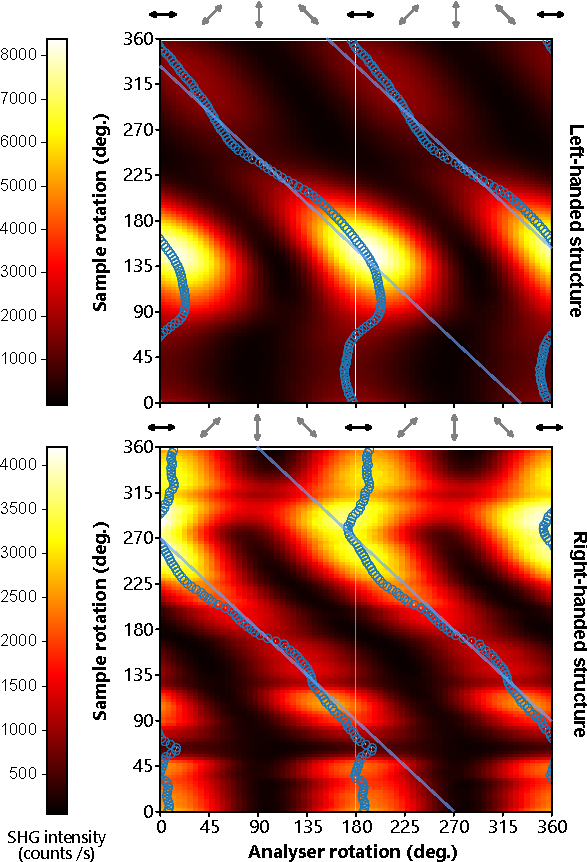
\includegraphics[scale=1]{./figures/results/OAinPlanarNanohelices/p_data.pdf}

    \caption{\label{fig:results:OAinPlanarNanohelices:p_data}
    SHG optical rotation heatmap for both enantiomorphs of the helical metamaterial, for P-polarised (parallel to the plane of incidence) incident light. In this case, both the angle of SHG-OR and the intensity of SHG emission are strongly dependent on sample rotation. Additionally, there is no clear reversal between enantiomorphs of the metamaterial. Instead, the sign of SHG-OR reverses under sample rotation, suggesting contributions from anisotropy dominating over contributions from the structure's intrinsic chirality.}	
\end{figure}

Importantly however, SHG-OR is not always independent of sample anisotropy. As discussed in section~\ref{sec:results:OAinPlanarNanohelices:discussion}, SHG is a highly symmetry-sensitive technique, whereby symmetry is expressed in the values of nonlinear susceptibility tensor elements. Depending on the experimental geometry, and on the values of these tensor elements, competing symmetries within the structure can be dominant in the measured results. This is directly demonstrated in figure~\ref{fig:results:OAinPlanarNanohelices:p_data}. 
The data presented in figure~\ref{fig:results:OAinPlanarNanohelices:p_data} were obtained from the same nanohelices, however whereas in figure~\ref{fig:results:OAinPlanarNanohelices:s_data} we used S-polarised light, here P-polarised light was employed. As in figure~\ref{fig:results:OAinPlanarNanohelices:s_data}, the heat maps correspond to SHG intensity as a function of sample and analyser rotation angles. Contrary to figure~\ref{fig:results:OAinPlanarNanohelices:s_data}, the SHG-OR angle changes significantly over the regions of SHG emission, closely following the sample rotation angle. This behaviour is exactly as expected for SHG-OR dominantly due to sample anisotropy. The experimental geometry must be carefully selected to address the structural chirality exclusively. 
Furthermore, additional data presented in Appendix~\ref{sec:appendix:AdditionalAuHelix} demonstrate that the precise experimental conditions required to isolate instrinsic chirality, and anisotropy, depend strongly on the geometry of the nanomaterial. We observe that changes in the nanohelix separation have a large impact on the nonlinear optical activity, entangling the effects of chirality and anisotropy. Changes in the nanohelix dimensions with the same separation have a less dramatic effect, preserving the anisotropy-dominated SHG-OR under p-polarised illumination, but also exhibiting no behaviour \textit{exclusively} attributable to chirality.

The nonlinear chiroptical behaviour reported here is in stark contrast to the linear chiroptical case. The linear OR of the nanohelices was investigated with optical microscopy and spectroscopy. 
Microscopy images were obtained on a commercial Zeiss Axio Imager M2m wide-field microscope, with a halogen lamp for illumination. Images were taken in bright-field reflection mode, through an Epiplan-Neofluar $20\times$/0.50 HD DIC objective, using an Axiocam 105 colour camera. Incident polarisation was controlled using a fixed Zeiss linear polariser slider, with the output image analysed with a Zeiss $\SI{360}{\deg}$ rotatable analyser slider. 
The analyser can be precisely rotated through $\SI{360}{\degree}$. Under crossed polariser geometry, only light that has experienced OR reaches the detector. By rotating the analyser, the sign of this OR can be obtained. 


Figure~\ref{fig:results:OAinPlanarNanohelices:lin_data}a shows a $3 \times 3$ array of optical microscopy images (in colour) of the nanohelices. The rows correspond to three different sample rotation angles ($\SI{0}{\degree}$, $\SI{45}{\degree}$ and $\SI{90}{\degree}$) and the columns corresponds to three analyser rotation angles ($\SI{85}{\degree}$, $\SI{90}{\degree}$, $\SI{95}{\degree}$).
The sign of OR is revealed by colour contrast in the images. For a sample oriented at $\SI{0}{\degree}$ and an analyser positioned at $\SI{85}{\degree}$, the image appears green.
Upon rotating the analyser to $\SI{95}{\degree}$, the colour changes to red. However, upon orienting the sample at $\SI{90}{\degree}$, the colour contrast reverses, indicating an opposite OR. This behaviour suggests that the angle of OR depends on sample orientation and that OR changes sign every $\SI{90}{\degree}$. 
This trend is confirmed in figure~\ref{fig:results:OAinPlanarNanohelices:lin_data}b, showing an OR spectral map, obtained by rotating the sample between crossed polarisers. 
Spectra were obtained by diverting the microscope image to a collection lens focusing onto a $\SI{400}{\micro\m}$ diameter multimode optical fibre. The output of the fibre was connected to an Ocean Optics QE Pro commercial spectrometer, running with a $\SI{500}{\milli\s}$ integration time. The spectral data is normalised to account for the spectral lineshape of our halogen lamp source. Reference spectra were obtained using a silver mirror to measure the spectral lineshape of the source only. The measured metamaterial spectra were divided by this reference to give spectra independent of the illumination source.
Here, a $\SI{90}{\degree}$ rotational periodicity for the OR is clearly visible, at wavelengths above $\SI{550}{\nano\m}$. The behaviour of the sample is consistent with that of a radiating dipole rotated through $\SI{360}{\degree}$. Such a dipole can be situated at the end-termination of the nanohelices. In the ranges of study, this dipole is excited by wavelengths from $\SI{550}{\nano\m}$ to $\SI{800}{\nano\m}$. The latter is the fundamental wavelength used for the SHG data in Figures~\ref{fig:results:OAinPlanarNanohelices:s_data} and~\ref{fig:results:OAinPlanarNanohelices:p_data}, where the SHG intensity also depends on coupling to the end-termination dipole, as discussed above.

\begin{figure}[htb!]	
    \centering	
    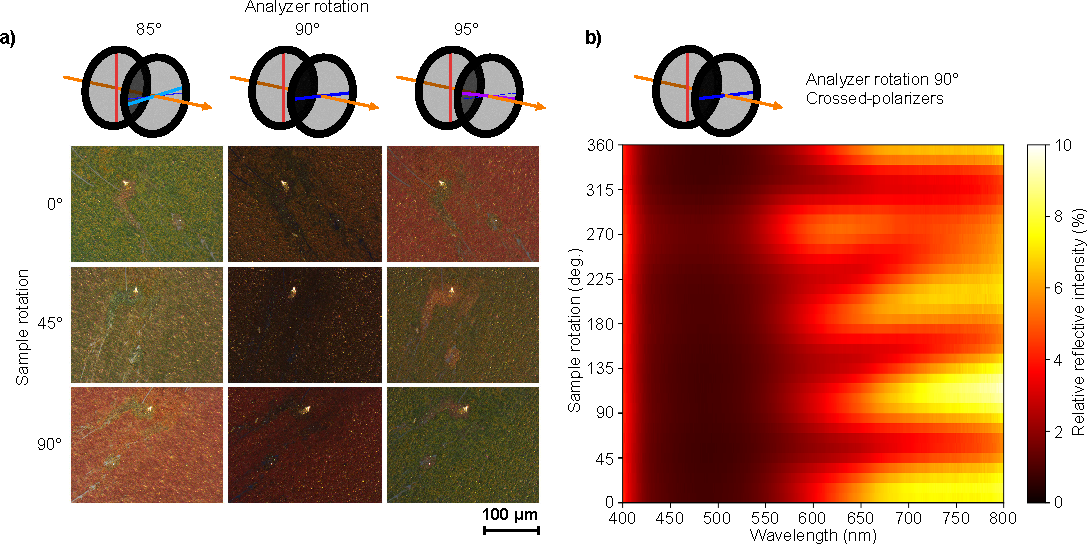
\includegraphics[scale=1]{./figures/results/OAinPlanarNanohelices/lin_data.pdf}

    \caption{\label{fig:results:OAinPlanarNanohelices:lin_data}
    Linear optical rotation data obtained through microscopy. \textbf{a)} Microscopy images of left-handed structure under illumination by linearly polarised white light, with various almost-crossed analysing polariser angles. By rotating the analyser slightly away from crossed ($\SI{90}{\degree}$), the spectral dependence of optical rotation can be observed. Longer wavelengths are transmitted more through the analyser when oriented at $+\SI{5}{\degree}$ away from crossed. Upon rotating the structure by $\SI{90}{\degree}$ the OR reverses. \textbf{b)} Linear OR map obtained from a spectrometer connected to the microscope viewport, showing clear dependence on sample rotation. Since the sample is between crossed polarisers, positive and negative OR both increase the measured intensity.}
\end{figure}

\section{Discussion}\label{sec:results:OAinPlanarNanohelices:discussion}
Due to the sub-wavelength dimensions and separation of nanostructure inclusions, our sample can be treated as an effective dielectric medium, described by effective susceptibility tensors as in section~\ref{sec:background:NonlinearOptics:susceptibility}.
At a given optical frequency $\omega$, the nonlinear chiroptical effects are described in terms of the nonlinear susceptibility tensors, relating the induced polarisation ($P$) at the second-harmonic ($2\omega$) to the driving electric ($E$) and magnetic ($B$) fields, by equation~\ref{eq:results:OAinPlanarNanohelices:P2contributions}.
\begin{equation}\label{eq:results:OAinPlanarNanohelices:P2contributions}	
    {P_i}\left( {2\omega } \right) = 
    \varepsilon{_0}\chi_{ijk}^{eee}{E_j}\left(\omega \right){E_k}\left(\omega \right) + \varepsilon{_0}\chi_{ijk}^{eem}{E_j}\left(\omega \right){B_k}\left(\omega \right) + \varepsilon{_0}\chi_{ijk}^{eme}{B_j}\left(\omega \right){E_k}\left(\omega \right)
\end{equation}
The indices $i$, $j$, and $k$ describe the Cartesian directions of the fields, and can represent $x$, $y$, or $z$ (see figure~\ref{fig:results:OAinPlanarNanohelices:setup}c). 
The superscripts $e$ and $m$ stand for electric and magnetic dipole transitions, respectively, while $\varepsilon{_0}$ is the permittivity of vacuum. 
In addition to equation~\ref{eq:results:OAinPlanarNanohelices:P2contributions}, the incident electromagnetic fields can induce a magnetisation $M_i$ analogous to the polarisation $P_i$. 
In our experiment (figure~\ref{fig:results:OAinPlanarNanohelices:s_data}), the incident electric field is polarised perpendicularly to the main helix axis, therefore this magnetic contribution is excluded. Away from resonance, the magnetic component of the incident light is much weaker than the electric component. 
In this analysis, only the contributions from electric dipoles ($eee$) are considered. Furthermore, for collinear SHG experiments, the incident fields ${E_j}(\omega)$ and ${E_k}(\omega)$ are indistinguishable. This allows equation~\ref{eq:results:OAinPlanarNanohelices:P2contributions} to be reduced under permutation symmetry as in section~\ref{sec:background:NonlinearOptics:permutation}.

The presence of spatial symmetry can further reduce the number of non-zero tensor components. The presence of surface isotropy (full rotational symmetry about the surface normal) would eliminate 11 components (section~\ref{sec:background:NonlinearOptics:rotation}). We can refer to these as the ``anisotropy components''. Likewise, for a tensor with mirror symmetry, 8 components are eliminated  (section~\ref{sec:background:NonlinearOptics:mirror}). These ``chirality components'' are therefore only present in chiral structures. Importantly, both anisotropy and chirality tensor components can contribute to SHG-OR. 

The nanohelix sample is a chiral, anisotropic surface. With S-polarised light, ${E_j}(\omega)$ and ${E_k}(\omega)$ are polarised along the sample $y$-axis. Therefore, only the $\chi_{xyy}$, $\chi_{yyy}$ and $\chi_{zyy}$ tensor components are addressed. Here, we examine each component individually. 
First, we can see that $\chi_{zyy}$ is neither an in-plane anisotropy, nor a chirality parameter. Second, $\chi_{yyy}$ is an anisotropy but not a chirality parameter. And third, $\chi_{xyy}$ relates to \textit{both} anisotropy and chirality. 
Rotating the sample by an angle $\theta$ around the surface normal is equivalent to applying a rotation operation to the $\chi_{ijk}(2\omega)$ tensor. The treatment can be simplified by introducing effective nonlinear susceptibility tensor components as given in equation~\ref{eq:results:OAinPlanarNanohelices:ChiEff}.

\begin{equation}\label{eq:results:OAinPlanarNanohelices:ChiEff}
	\begin{split}
		&\chi_{xyy}^{eff}(\theta) = \cos\theta\sin^2\theta(\chi_{xxx} - 2\chi_{yyx}) \\
		&+ {\cos^2}\theta\sin\theta (2\chi _{xyx} - \chi_{yyy}) + {\cos^3}\theta(\chi_{xyy}) - {\sin^3}\theta(\chi _{yxx}), \\
		\\
		&\chi_{yyy}^{eff}(\theta) = \cos\theta\sin^2\theta(2\chi_{xyx} - \chi_{yxx}) \\
		&+ {\cos^2}\theta\sin\theta (2\chi _{yyx} - \chi_{xyy}) + {\cos^3}\theta(\chi_{yyy}) - {\sin^3}\theta(\chi _{xxx}), \\
		\\
		&\chi _{zyy}^{eff}(\theta) = \cos\theta\sin\theta (2\chi_{zxy}) + {\sin^2}\theta(\chi_{zxx}) + {\cos^2}\theta (\chi_{zyy}).
	\end{split}
\end{equation}
Within the dipole approximation, the angle of SHG-OR is $\phi=\arctan{\left(\frac{E_P\left(2\omega\right)}{E_S\left(2\omega\right)}\right)}$. 
The values of the electric fields at the second harmonic are obtained from ${\mathbf{E}(2\omega)\sim[\mathbf{n}\times\mathbf{P}(2\omega)]\times\mathbf{n}}$, where $\mathbf{P}(2\omega)$ is a vector describing the induced polarisation, and $\mathbf{n}$ is a unit vector describing the angle of observation. 
In our experimental configuration, the angle of optical incidence is $\SI{45}{\degree}$, hence $E_P(2\omega)\propto\frac{1}{2}(\chi_{zyy}^{eff}(\theta)-\chi_{xyy}^{eff}(\theta))$ and $E_P(2\omega)\propto\chi_{yyy}^{eff}(\theta)$. 
The angle of SHG-OR in this configuration is therefore given by equation~\ref{eq:results:OAinPlanarNanohelices:SHGangle}.
\begin{equation}\label{eq:results:OAinPlanarNanohelices:SHGangle}
	\phi  = \arctan \left({\frac{\chi_{zyy}^{eff}(\theta) - \chi _{xyy}^{eff}(\theta)}{2\chi _{yyy}^{eff}(\theta)}}\right)
\end{equation}
Likewise, the intensity of SHG emission is given by equation~\ref{eq:results:OAinPlanarNanohelices:SHGintensity}.
\begin{equation}\label{eq:results:OAinPlanarNanohelices:SHGintensity}
	I_{SHG} \propto \frac{1}{4}{\left| {\chi _{zyy}^{eff}\left( \theta  \right) - \chi _{xyy}^{eff}\left( \theta  \right)} \right|^2} + {\left| {\chi _{yyy}^{eff}\left( \theta  \right)} \right|^2}
\end{equation}
Although not trivial, the effects of anisotropy and chirality can be disentangled. To achieve this, equation~\ref{eq:results:OAinPlanarNanohelices:ExampleComponents} presents a suitable set of intrinsic tensor component relationships, as an example.
\begin{equation}\label{eq:results:OAinPlanarNanohelices:ExampleComponents}
	\begin{split}
		& \chi_{xxx} = \pm 0.5; \chi_{xyy} = \mp0.58; \chi_{yyx} = \pm 0.55 \\
		& \chi _{yxx} = 1.0; \chi _{yyy} = 0.34; \chi _{zyy} = 0.05; \chi _{zxx} = 0.02; \chi_{zyy} = 0.05; \chi _{zyx} = 0.01
	\end{split}
\end{equation}
The top three tensor components are pseudo-scalars associated with chirality, and thus change sign depending on the handedness of the structure ($+$ and $-$ for left- and right-handed structures, respectively). 
The lower 6 tensor components describe structural anisotropy, and do not change sign under parity inversion. 
With the values in equation~\ref{eq:results:OAinPlanarNanohelices:ExampleComponents}, we can calculate the SHG intensity and SHG-OR, for both enantiomorphs, see Figure~\ref{fig:results:OAinPlanarNanohelices:sim_data}. 
The figure has the same layout as Figure~\ref{fig:results:OAinPlanarNanohelices:s_data} and it can be seen that it matches very well the experimental behaviour. 
\begin{figure}[htb!]	
    \centering	
    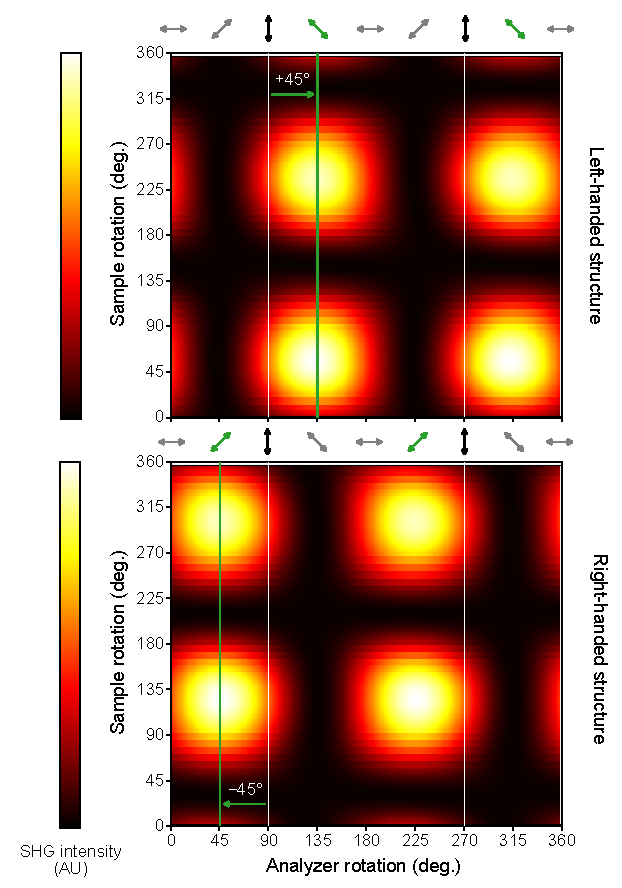
\includegraphics[scale=1]{./figures/results/OAinPlanarNanohelices/sim_data.pdf}

    \caption{\label{fig:results:OAinPlanarNanohelices:sim_data}
    SHG optical rotation heatmaps for the susceptibility tensor relationships given in equation~\ref{eq:results:OAinPlanarNanohelices:ExampleComponents}. The SHG-OR behaviour closely matches that observed in Figure~\ref{fig:results:OAinPlanarNanohelices:s_data}.}
\end{figure}

In an \textit{isotropic} metasurface, composed of nanohelices, two principal models can be used to theoretically quantify the nonlinear optical activity. The first model builds upon Kauzmann's ``one-electron chirality''~\cite{Kauzmann1957a}.
In its nonlinear treatment, the nonlinear optical activity requires magnetic dipoles caused by the electron's helical motion~\cite{Maki1996, Hache2001a}.
The second model, builds upon Kuhn's~\cite{Kuhn1930} chirally-coupled electric dipole moments. In its nonlinear treatment, the nonlinear optical. activity requires only electric dipole moments~\cite{Hache2001a}.
In plasmonic nanomaterials this could be the coupling between any chirally-arranged metallic features. Importantly, the ``one-electron'' model permits only SHG-CID, whereas the coupled-dipole model allows SHG-CID, SHG linear dichroism (SHG-LD), and SHG-OR~\cite{Fischer2005a}.
Unlike linear chiroptical measurements, information is gained by measuring both SHG-CID and SHG-OR: the mechanism of a structure's chiroptical response can be determined by comparing these two nonlinear chiroptical effects. 

However, when treating \textit{anisotropic} surfaces, the analysis is much more complex than in the isotropic case. SHG-OR is possible in both models, and there is no simple distinction between the two. Slight changes in the structure design can result in significant changes in the optical behaviour, due to the large number of interacting tensor components responsible for the SHG-OR. As we have observed, this complexity can result in interesting and highly desirable optical properties, under the right experimental and geometric conditions. The flexibility of geometry makes metamaterials an ideal platform for exploring this interplay between structural and experimental geometry. 

Finally, it is important to consider that the SHG-OR in Figure~\ref{fig:results:OAinPlanarNanohelices:s_data} could, in principle, originate from the out of plane anisotropy axis. SHG-OR effects from this axis would not change under azimuthal sample rotation. However, such an anisotropy-induced SHG-OR would not change sign, depending on the handedness of the nanohelices. Consequently, because our SHG-OR changes sign depending on handedness, we can conclusively attribute it to chirality. 

\section{Conclusions}\label{sec:results:OAinPlanarNanohelices:conclusions}
To conclude, this chapter reports a large SHG-OR effect of $\pm \SI{45}{\deg}$ from planar chiral metamaterials. The effect is due to the intrinsic chirality of the helical nanostructures; the angle of SHG-OR is rotationally invariant, and, as expected, it reverses for the mirrored structures. Contrary to their linear chiroptical counterparts, SHG-CID and SHG-OR are not trivially related to one another. Therefore, these results pertain to an important and previously unobserved chiroptical effect in this kind of system. We have demonstrated that, under specific experimental conditions, it is possible to extract purely chiral information from highly anisotropic structures. Further work on disentangling chiral and anisotropic contributions to nonlinear chiroptical effects will unveil the physical mechanisms at work and will lead to their optimisation. 